\documentclass[11pt,a4paper]{article}

\usepackage{main}
\usepackage{cours}

\renewcommand{\typedocument}{Cours}
\renewcommand{\classe}{6e}
\renewcommand{\titre}{Schémas de chaîne énergétique}

\begin{document}

\creertitre{Schémas de chaîne énergétique}

Pour représenter une conversion d’énergie, on dessine un schéma de chaîne d’énergie :

\begin{itemize}
    \item On dessine les \textcolor{orange}{convertisseurs d’énergie} dans des rectangles
    \item On dessine les \textcolor{violet}{énergies} avec des flèches. L'énergie utilisée par le convertisseur est représentée par une flèche qui pointe vers le convertisseur, et les énergies produites sont représentées par des flèches qui partent du convertisseur.
\end{itemize}

\uline{Méthodologie}:

\begin{enumerate}
    \item Identifier les convertisseurs d'énergie,
    \item Identifier les énergies utilisées et produites par chaque convertisseur,
    \item Dessiner les rectangles pour les convertisseurs,
    \item Dessiner les flèches pour les énergies, en indiquant la forme d'énergie.
\end{enumerate}

\exemple{Un \textcolor{orange}{ventilateur} utilise de l’\textcolor{violet}{électricité} pour mettre de l’air en \textcolor{violet}{mouvement}. Le ventilateur \textcolor{violet}{chauffe} lorsqu’il fonctionne.}

\begin{center}
    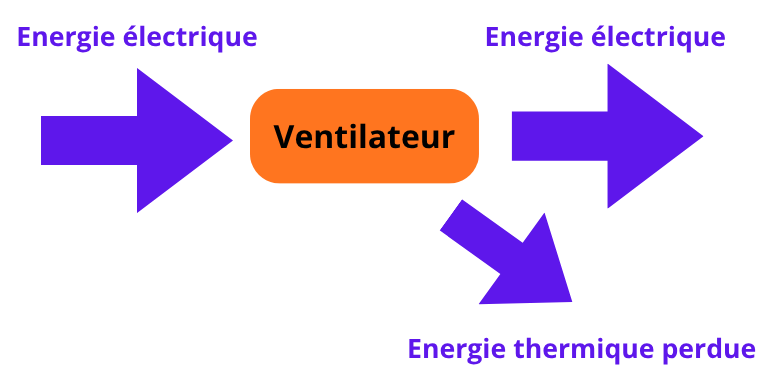
\includegraphics[width=14cm]{images/chaine_energetique.png}
\end{center}

\end{document}